\chapter{Бочка}
%\corner{64}
\vepsianrose

Проснулись пацаны поздно\mdash утро было пасмурным и сонным, да и вчера засиделись. Костёр долго не хотел разгораться, все ощущали невыносимую леность. Адмирал решил приготовить на завтрак пшёнку с изюмом на сгущенке и сливках. Каша вышла\mdash класс. Команда, как обычно расселась вокруг костра и трапезничала:

\diagdash Шу-у-урик, от пуза.\mdash Серёга звенел ложкой по~тарелке.

\diagdash Ну.

\diagdash Изюма не поскупился.\mdash Замполит уминал за обе щеки.

\diagdash Ты ж меня знаешь!\mdash Адмирал развалился в~походном кресле и попивал чаёк.\mdash Насчёт голодать в~походе\mdash это не про меня.

\begin{wrapfigure}[12]{l}{0.48\textwidth}
	%\begin{figure}[h]
	\centering
	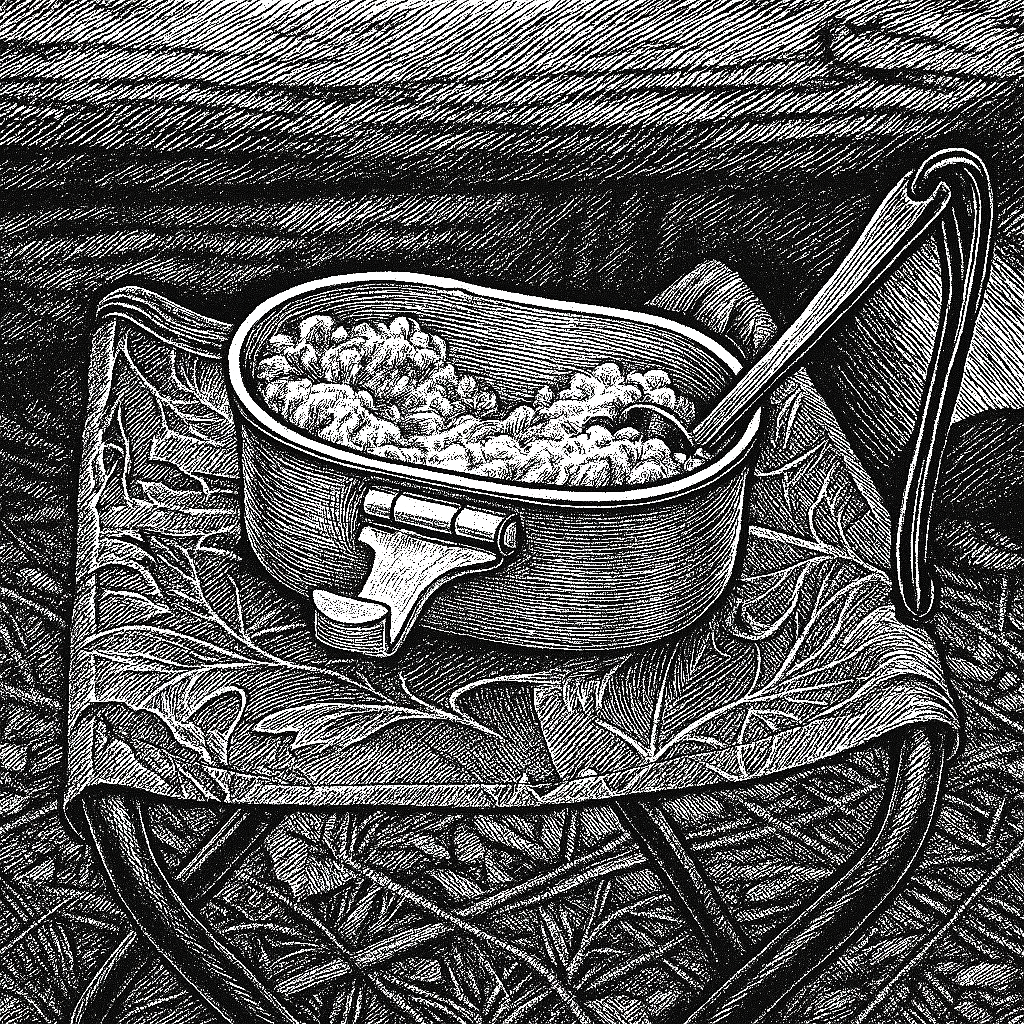
\includegraphics[width=0.45\textwidth]{44_1_porridge}
	\caption{\small\textit{...пшёнка с изюмом...}}
	%\end{figure}
\end{wrapfigure}
\diagdash Сань, чё у нас сегодня?\mdash Паша покончил с~кашей и~достал конфеты к~чаю.

\diagdash Вчера обсуждали вродь как. Сегодня\mdash ещё 4 порога последних и дальше по широкой Суне почти до~Викшозера. Кирь, доставай описание порогов\mdash самое время освежить в~памяти.

\diagdash Дай доесть?\mdash тот сидел в жёлтом дождевике на~бревне и был ещё вовсю занят пшёнкой.

\diagdash Давай-давай! Всё в темпе надо бы, уже к полудню времячко\sdash то.

Наконец Замполит добил завтрак и достал мобильник, открыл описание:

\diagdash Так, ну вот$\ldots$ <<Порог Длинный, 3 к.с.>>$\ldots$\mdash Киря оторвал глаза от телефона,\mdash $\ldots$Что это за нахрен? Откуда тройка?

\diagdash Врут. Маршрут заявлен как второй категории. Читай давай.\mdash Адмирал открыл карту в планшете.

\diagdash Да хрен знает! Может из\sdash за одного порога третьей категории не стали поднимать сложность всего маршрута? 

\diagdash Кирь, хар\'ош! Читай.

\diagdash <<$\ldots$В высокую воду это ключевое препятствие нижней части Суны>>$\ldots$ Э-э-э$\ldots$ %Да твою ж налево, Шурик!

\diagdash Ну, вода у нас высокая, как мы поняли. Ты~читай\sdash читай.\mdash ребята сидели в кружок у костра и~слушали.

\diagdash <<Основная струя оттесняется влево плитой в~центре, образуя$\ldots$>>\mdash так, ну это ерунда\mdash <<$\ldots$крутые метровые валы>>. Ага. Дальше <<$\ldots$после бочки за плитой лучше уходить вправо, в просвет между основной струей и~отбойными валами у правого берега>>.\mdash Замполит поднял полный укоризны взгляд.\mdash Шурик, опять <<бочка>>!

\diagdash Подытожим. Пишут, что это самый сложный порог на реке. Вода у нас высокая, как мы поняли уже с~вами. Итак, <<бочка>> опять где\sdash то за плитой. Прошлую мы с вами не заметили, а тут как пойдё\sdash ё\sdash ёт.\mdash протянул своё любимое Адмирал.

\diagdash Так. А что ещё пишут?\mdash спросили Серёга с~Русланом.

Замполит бегло почитал дальше и огласил:

\diagdash Ну тут альтернативный путь прохождения есть\mdash пишут, что надо прижиматься к невысоким сливам справа$\ldots$

\diagdash Это уже хрен с ним\mdash раз есть альтернатива, то~не~всё так страшно, на воде сориентируемся. Ты про <<бочку>> ещё разок почитай, п\sdash жалста.

\diagdash <<$\ldots$Струя оттесняется влево плитой в центре>>, а~дальше <<после бочки за плитой, лучше уходить вправо>>. Во-о-от.

\diagdash Итак, плита в центре, за ней <<бочка>>, обходить справа. Так?

\diagdash Ну да$\ldots$\mdash неуверенно отозвался Замполит.

\diagdash Все запомнили?\mdash Адмирал оглядел команду.

\diagdash Угу!\mdash Пашка наклонился к костру и бросил в пламя фантики от конфет.

\diagdash Длина какая у всего этого?\mdash уточнил Адмирал.

\diagdash Километр двести.\mdash отозвался Замполит.

\diagdash Ну на то и <<Длинный>>! Явно не короткий.\mdash поязвил Серёга.

\diagdash Нормас. Дальше бегленько прочитай про остальные и начинаем паковаться.\mdash сказал Адмирал, чтобы отвлечь взбудораженную команду от мыслей о <<бочке>>.

Замполит продолжил:

\diagdash Дальше Корбикоски без особых каких\sdash то проблем. Потом порог Блин, где пишут, что можно сигануть с~плиты у~правого берега. Та\sdash а\sdash ак. Потом ещё один порог и~последний\mdash Ледяной, где никакой жести$\ldots$

\diagdash Кирь, на карте Блина нет, но есть Руозмикоски, я~помню там какая\sdash то путаница была в описаниях.\mdash Адмирал посмотрел на карту.

\diagdash Хм! Походу Блин\mdash это и есть Руозми\sdash что\sdash то там?\diagdash предположил Серёга.

\diagdash Руозмикоски. Ну или это первая или последняя ступень, соответственно, последующего или предыдущего порога. Короче так, давайте сначала Длинный пройдём, а~дальше по~ситуации?

\diagdash Ладно, про <<бочку>> уяснили, дальше всё равно ничё не запомним.\mdash заключил Паша.

\diagdash Пакуемся!\mdash распорядился Адмирал$\ldots$

\vspace{0.5cm}
$\ldots$На воду они встали уже когда перевалило за~12~часов. Со стоянки на острове не хотелось уходить\mdash вроде бы, на~первый взгляд с воды, неуютный берег открывался чудесной поляной у костра с завораживающими соснами и елями вокруг. Эдакое <<потайное>> место, открывшееся, вероятно, в~первый раз тем, кто не гнушался основательно вести разведку стоянок. Адмиралу вдруг подумалось\mdash а~как вообще люди ходили по маршрутам когда не было ни навигации спутниковой, ни нормальных карт, ни толком описания? Наверняка кто\sdash то когда\sdash то пошёл первым, да хоть и по их маршруту по Суне, на байдарках типа <<Салют>> или ещё чёрт знает на чём самодельном в отрыв от окружающей действительности и принёс первый отчёт по маршруту. Это~если <<по\sdash официальному>> от какого\sdash нибудь турклуба. А если <<дикарями>>, как они? <<Непостижимо, как люди не боялись идти в неизвестность порогов, не имея чёткого понимания о~них>>,\mdash думал Адмирал,\mdash <<и если уж они сдюжили, то мы\sdash то~просто обязаны. Кроме того, наверняка местное население веками ловило тут рыбу на порогах>>.

Замполит залил костёр и осмотрел стоянку:

\diagdash Готово дело, уходим! Шурик, готов?

\diagdash Готов. Осмотритесь как следует! Тут трава высокая, может что забыли или выронили. Ну и отчаливаем.\mdash и~пошёл к~берегу.

На берегу Руслан в своей сиреневой болоневой курточке помогал Паше доканчивать погрузку. Адмирал закатал штанины, зашёл в воду и докончил погрузку своей байды, закрыв грузовой отсек заглушкой и как можно туже завязав шнур, стягивающий эту самую заглушку. Все собрались на~берегу и были готовы. 

\diagdash Отчаливаем!\mdash велел Адмирал, садясь в~байдарку.

\diagdash Ага!\mdash отозвалась команда.

\diagdash Начинаем потихонечку. Помним, что~далеко не~расходимся, радиосвязи нет~больше.

%\diagdash Ага-ага, ты давай первым, а~мы за~тобой.\mdash сказал Замполит.
\diagdash Ты давай первым, а~мы за~тобой.\mdash сказал Замполит.

\diagdash По классике, так сказать. Давайте, начали! Помним, <<бочка>> где\sdash то по центру, обходить справа.\mdash и Адмирал оттолкнулся от~берега веслом.

Две байдарки вышли в разлив после порога Каданлоама и дрейфовали\mdash все застёгивали юбки, проверяли замки спасжилетов, морально готовились. Миновав то место, откуда вчера удирали от засасывающего течения, они завернули за поворот реки и Длинный или, как ещё было в скобочках уточнено на адмиральской карте, Каменный, начался.

Последовало сужение русла, впереди выросли огроменные валы, Адмирал похолодел, но проходить\sdash то как\sdash то надо было, и направил их байдарку аккурат в валы, стараясь заходить максимально перпендикулярно к ним:

\diagdash {\large НА ВАЛЫ! РОВНО!}\mdash заорал Адмирал, а сам приготовился табанить для возможных манёвров.

БАХ! И вода залила Пашку, Руслана, окатила Адмирала на корме. БАХ!!! Ещё один вал. БАХ!!!!!! Ещё и~ещё! Высоченные валы они миновали отделавшись только лёгким испугом и брызгами. Дальше началась какая\sdash то сплошняковая белая каша воды. 

Экипаж молчал, а Адмирал соображал куда править дальше. Улучив момент, он обернулся и увидел, что Замполит заходит следом за ними в отдалении метров 50. Впереди начиналось очередное сужение, струя стремнины по центру косо уходила к правому берегу. <<Ага, там рекомендовали под правый берег>>,\mdash вспомнил Адмирал и взял чуть правее, довольный собой, думая как он сейчас обойдёт бурлящую кашу, что~была по центру и левее в русле. Справа по~курсу начинались прибрежные камни, и он молниеносно подправил их байдарку в такой узенький <<коридорчик>> между правым берегом и~косой стремниной$\ldots$ и тут же осознал, что~происходит\mdash их утягивало течением прямиком в <<бочку>>. Адмирал увидал ту самую плиту, о которой они прочли в~описании порога. За плитой стал виден водопад с бешеным бурлением, где притаилась коварная <<бочка>>. Скорость у них была аховая, всё это случилось настолько быстро, что Адмирал только и~успел, что рот открыть, чтоб заорать что\sdash нибудь матерное на~прощание, и~в~этот самый момент они рубанули байдаркой прямо по плите, почувствовался скользящий удар в днище, и~корабль носом зарылся в~<<бочку>>.

%\begin{wrapfigure}[12]{r}{0.48\textwidth}
%%	\begin{figure}[h]
%	\centering
%	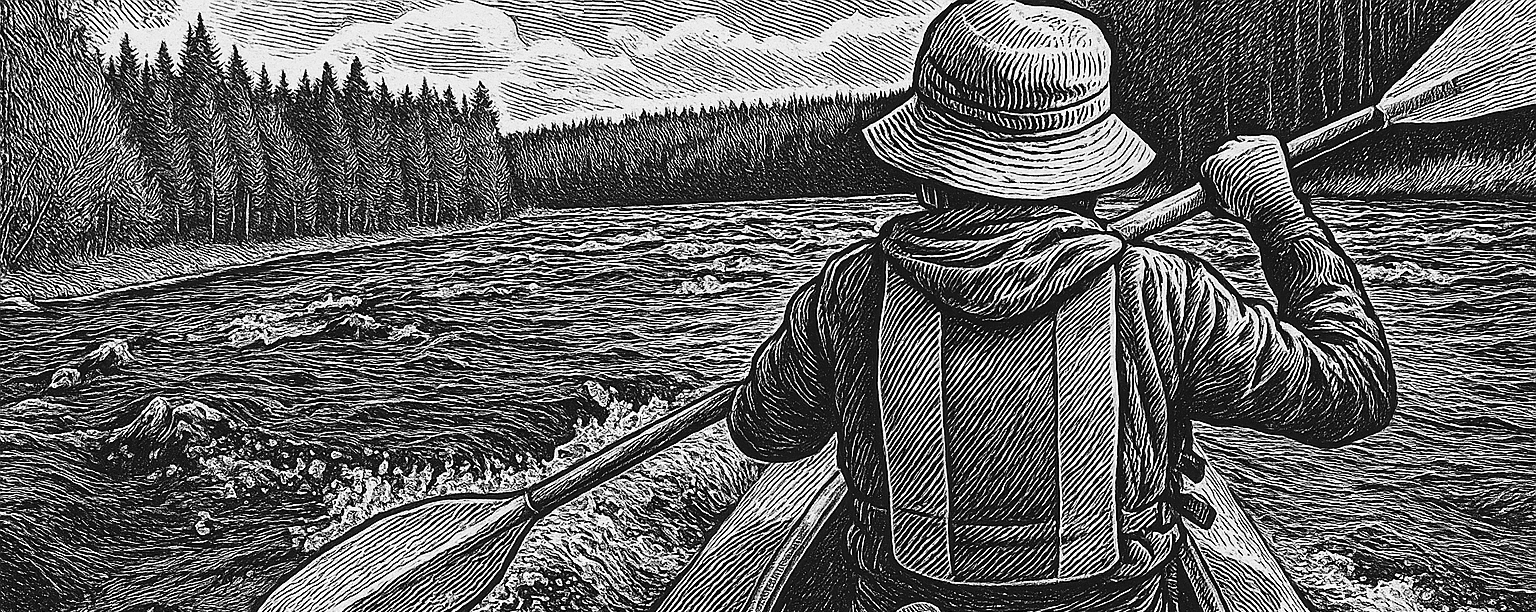
\includegraphics[width=1.0\textwidth]{bochka}
%	\caption{\small\textit{...рубанули байдаркой прямо по плите...}}
%%	\end{figure}
%\end{wrapfigure}

\diagdash {\LARGE ГРЕБЁМ!!!}\mdash бешено лопатя веслом, орал Адмирал. Ужас, обуявший его, просто не поддаётся описанию. Их байдарка, как в замедленном видео, чирканув 

%\begin{wrapfigure}{c}{1.0\textwidth}
		\begin{figure}[h]
		\centering
		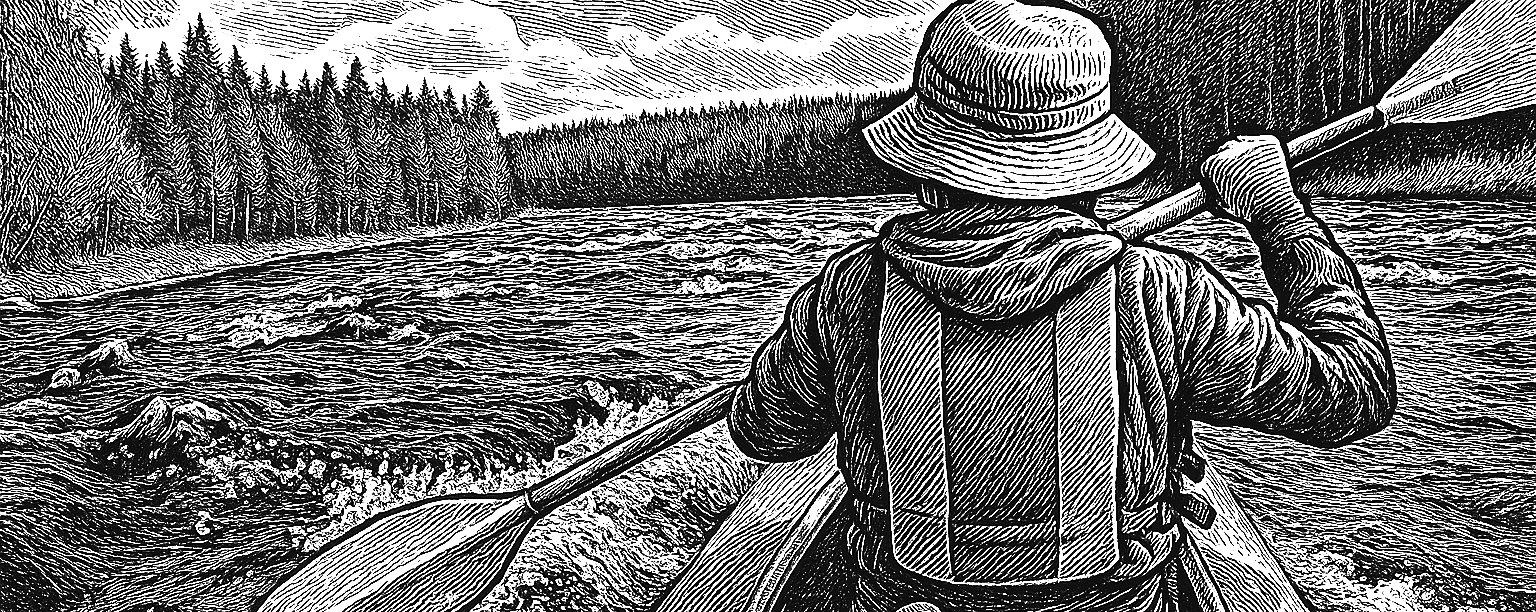
\includegraphics[width=1.0\textwidth]{45_1_bochka}
		\caption{\small\textit{...рубанули байдаркой прямо по плите...}}
		\end{figure}
%\end{wrapfigure} 

\noindent днищем по каменной плите, угодила в самую середину того, что при низкой воде могло бы быть довольно злой <<бочкой>>. Но скорость была высока, и это спасло их\mdash они, бешено лопатя вёслами, вышли из порога:%пены победителями.

\diagdash Фу-у-ух, пронесло, кажись!\mdash Пашка сел повыше.

\diagdash Горе-сплавщики, ёклмн-ёпрст!

\diagdash Не, ну она из ниоткуда появилась!\mdash пошли толки.

\diagdash На дно смотрите, воды не прибывает?! Удар\sdash то неслабый был.\mdash Адмирал открыл юбку и заглянул в трюм.%Адмирал открыл юбку и окинул взглядом трюм.

\diagdash Да вроде не хлещет$\ldots$\mdash отозвался экипаж.

\diagdash Ладно, как там Киря?\mdash Адмирал погасил скорость табаном и улучил момент обернуться назад в надежде, что Замполит догадается обойти эту плиту. Махать второму экипажу веслом или орать было бесполезно\mdash всё равно бы ничего не~услышали из\sdash за шума воды или не поняли бы. 

Минуту спустя Замполит не подвёл\mdash повторяя траекторию Адмирала, он тоже ломанулся на плиту и угодил в <<бочку>>. До адмиральского экипажа сквозь рёв стихии донеслись вопли отчаянной борьбы, а мгновения спустя\mdash дикий истерический хохот:

\diagdash Профессионалы, ёпт!!!\mdash Киря пронёсся мимо них.

\diagdash Тащ Замполит, поздравляю с <<профессиональным>> прохождением <<бочки>>.\mdash ёрничал Адмирал.

\diagdash Шурик!!! Мы на вас ориентировались! Я не сразу понял, что вы влипли, а потом, когда понял, уже поздно было$\ldots$\mdash начал было Замполит.

\diagdash Кирь, ты не поверишь, такая же фигня! Вот прям один\sdash в\sdash один\mdash когда поняли, что влипли, было поздно!

Серёге, Руслану и Паше ничего не оставалось, как словесно посетовать на нерадивых капитанов, проведших их по самой, так сказать, жести порога:

\diagdash Профи, чё. Сразу видно.

\diagdash Так, аллё! Бунтовщиков утоплю. Готовимся к~Корбикоски$\ldots$

Корбикоски им ничем не запомнился, поскольку показался скорее лёгкой шиверой после Длинного. Они быстро приближались к следующему порогу, Руозмикоски. Замполит распевал:

\diagdash Всё перекаты, да перекаты, послать бы их па\sdash а\sdash а а\sdash а\sdash адресу!

\diagdash На это место уж нету ка\sdash а\sdash арты, плывём вперёд по~абрису\sdash у\sdash у!\mdash подхватил Адмирал.

\diagdash Шу-у-урик, куда?\mdash Серёга и Киря шли впереди адмиральской трёшки. Впереди виднелся островок в~начале порога. Адмирал медлил, стараясь наметить путь прохождения поспокойнее.

\diagdash Так, парни, слушай мою команду! Островок огибаем слева, прижимаясь к прибрежной траве, а потом резко под правый берег\mdash вслед за рыбаками!\mdash заорал Адмирал, увидав в пороге две надувные моторки, на которых было по~одному мужику. Рыбаки проходили Руозмикоски стоя, ловко управляя разрезными вёслами. Моторы, естественно, были~подняты.

\diagdash Давай вперёд!\mdash Замполит пропустил адмиральский экипаж и встал в кильватер. Впрочем, совсем скоро кильватер превратился во что\sdash угодно\sdash ватер, когда сила стихии начала швырять их судёнышки по валам.

Адмирал увидел, что мужики на моторках, которые беспорядочно колбасило на волнах, прибиваются к правому берегу, где было поспокойнее. Не став повторять их заход, Адмирал ломанулся прямо по <<языку>> в самую середину. Лавируя по руслу между камнями, он понял, что это была лишь прелюдия\mdash его взору открылась вторая ступень порога с мощным широким сливом. Моторочники, балансируя на~ногах, ушли под самый правый берег, а~Адмирал опять пошёл ближе к центру, пройдя по гребням чуть правее самых больших валов. 

\diagdash А недурно, парни, а?\mdash довольный Адмирал обернулся поглядеть вверх по течению на~порог.

\diagdash Ску-у-чно уже,\mdash отозвался Паша.\mdash не~то, что~вчера.

\diagdash Ну не знаю, по\sdash моему норм.\mdash ответил Руслан.

\diagdash Гляньте, стояночка! И~навес деревянный, оп\sdash па.\mdash Адмирал увидал хорошую добротную стоянку и~немедленно решил причалить к~левому берегу.

Пристав к берегу и подзатащив байду на песочек, адмиральский экипаж стал ожидать Замполита. Те подошли буквально через пару минут, отстав на входе в порог от~Адмирала:

\diagdash Стояночка\sdash то класс!\mdash Замполит пошёл оглядеться.

\diagdash Да, но становиться\mdash ещё рано.\mdash Адмирал развязал вещмешок и достал батончики спортпита на всех.

\diagdash Шу-у-урик, пойдём порог сфоткаем?\mdash Серёга, взяв батончик, собрался пойти выше по течению берегом.

\diagdash Не, нафиг.\mdash Адмирал пошёл исследовать навес и~стоянку, а Серёга пошёл фоткать порог в одиночестве. 

Команда разбрелась по берегу. Адмирал заценил расположение и красоту стоянки прямо за порогом. Он~подошёл к навесу. Тот был весь исписан автографами сплавщиков\mdash города, имена, даты$\ldots$

\diagdash Зацените!\mdash показал Адмирал подошедшей команде.

\diagdash Впишемся?\mdash предложил Руслан.

\diagdash Лень за ручкой идти$\ldots$

\vspace{0.5cm}
$\ldots$Погуляв по берегу, ребята доели батончики, выпили чаю и снова встали на воду:

\diagdash Сань, чё дальше?

\diagdash Последний порог\mdash Ледяной.

\diagdash Название так себе.\mdash резюмировал Серёга.

\diagdash <<Крайний>> надо говорить, ну?\mdash иронизировал Паша.

\diagdash Да не, там пишут лёгкая шивера, правда с~обливняками, я почитал на перекусе.\mdash ответил Адмирал, и эскадра без проблем преодолела последний порог шиверистого типа, действительно лавируя меж камней. Слева впала небольшая речушка.

\diagdash Шурик, как называется?\mdash Замполит обгонял адмиральский экипаж.

\diagdash Ручей? Деяоя.

\diagdash Чё?!

\diagdash Так написано на карте, Кирь. Всё, после впадения этого ручья порогов нет, мы прошли активную часть маршрута, парни, с чем я вас и поздравляю!

%\begin{wrapfigure}{c}{1.0\textwidth}
\begin{figure}[h]
	\centering
	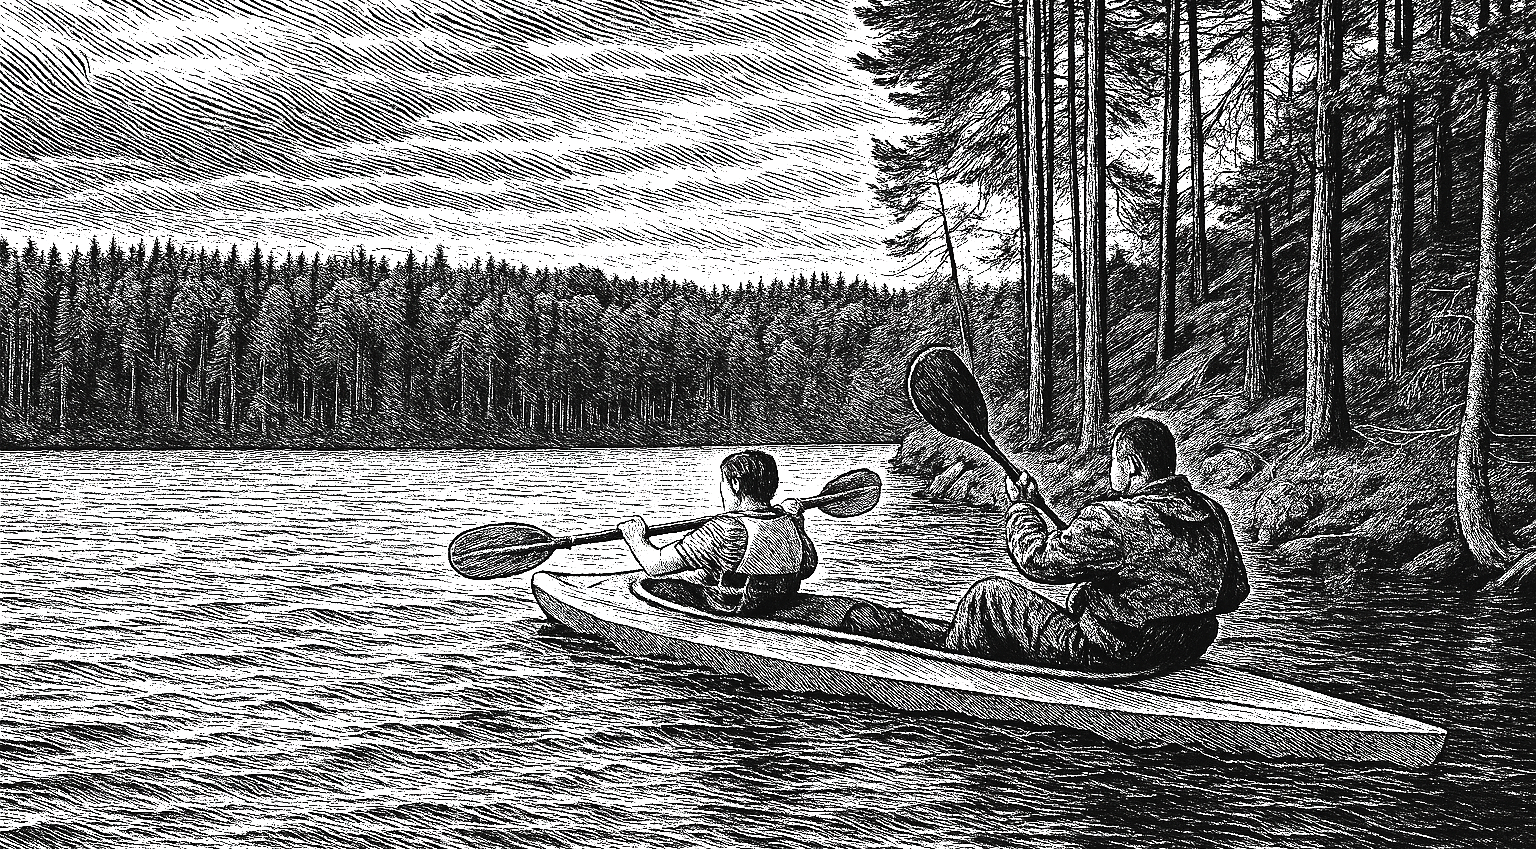
\includegraphics[width=1.0\textwidth]{46_1_endporogs}
	\caption{\small\textit{...пороги кончились...}}
\end{figure}
%\end{wrapfigure} 

Пороги закончились. Река стала заметно шире, полноводнее, течение замедлилось. Левый берег был довольно крутым, откосы доходили до 45 градусов. Виднелись следы низового пожара\mdash стволы почернели, землю устилала гарь. Верхушки сосен при этом стояли незадетыми. Правый берег был пониже и утопал в~лиственной растительности. 

Впереди слева замаячила большая скала, выдающаяся из крутого берега в реку. <<Ага, видимо про неё я читал, что там должна быть стоянка.>>\mdash подумал Адмирал и~спустя пару мгновений убедился в этом\mdash место было занято большой группой сплавщиков, расположившихся на скале.

\diagdash Коммерческие.\mdash резюмировал Паша.\mdash вон у них там флаг и всё такое. Это мы их вчера обгоняли.

\diagdash Ну классика\mdash фиг щас мы тут стоянку найдём.\mdash раздосадованно сказал Замполит.

\diagdash Найдём, не боись. Времени навалом.\mdash Адмирал поглядел на свои китайские ролексы\mdash времени едва перевалило за 3 пополудни.

Спустя ещё немного времени берега поменялись местами\mdash левый стал низким, откосы пошли справа. Они вошли в своеобразную <<воронку>> русла, поднялся попутный ветер. Замполит лопатил где\sdash то впереди.

\diagdash Паш, ставь парус.\mdash Адмиралу хотелось отдохнуть от гребли и расслабиться.

\diagdash Ага!\mdash тот немедленно приладил к веслу их парус, байду потащило.

\diagdash Вот это я понимаю! Ка-а-айф, мужики.

\diagdash Да-а-а!\mdash Адмирал взял весло под мышку, закурил папиросу и, облокотившись на борт, попробовал развалиться как можно вальяжнее, насколько это вообще было возможно. 

Ветер дул, конечно, не совсем попутный\mdash их сносило к левому берегу, отчего Адмирал с Русланом изредко подправляли курс. На крутых откосах правого берега они прошли ещё одну занятую стоянку. Адмирал приподнял панаму и поздоровался с людьми, которые восторженно приветствовали адмиральскую трёшку, вовсю рассекающую водную гладь под полусферическим парусом.

Замполит грёб впереди адмиральского экипажа, упахиваясь и высоко поднимая лопасти весла. Адмирал же, развалившись с папироской, только подправлял курс и~откровенно кайфовал от происходящего\mdash мощный сильный ветер тащил их вперёд так, что одного только паруса было достаточно, чтобы не отставать от Кири, который неслабо лопатил, не желая идти вторым. <<Фантастика>>,\mdash думалось Адмиралу о парусе.\mdash<<Гениальнейшее изобретение человечества. Надо строить парусник, однозначно>>.

Спустя километра четыре после Ледяного, пройдя плавные изгибы русла широкой Суны, ребята попробовали разведать стоянку на левом и правом берегах, разделившись. Места не нравились. Им хотелось прям вау\sdash стоянки, а такие, как назло, или не попадались, или были заняты.

Замполитовский экипаж разведал местечко по левому берегу, но оставаться там Адмирал не захотел, полагая идти на поиски дальше, к новым красотам реки, подумав, что, быть может, в устье Семчи, впадающей в Суну слева, удача улыбнётся им:

\diagdash Давайте разведаем тут.\mdash сказал Адмирал, развернувшись против течения и подойдя к довольно таки обрывистому каменистому правому бережку.

\diagdash Выхода нет нормального к воде, супер\sdash места не будет, стопроц.\mdash начал Замполит.

\diagdash Ну хоть разомнём ноги.\mdash Паша свернул парус, и~маленькая эскадра пристала к камням.

Они оказались почти на самом мысу у впадения Семчи. Адмирал был просто уверен, что тут обязана быть неземных красот стоянка. Место было действительно очень красивым\mdash каменистый склон с выходом скальных пород зарос высоченными соснами, под ногами рассыпался мшаник вперемешку с камнями. Уклон берега был переменным\mdash то вверх, то вниз, отчего ровного места под палатки и хозчасть практически не было.

\diagdash Шурик, ну не алё.\mdash заключил Замполит.

\diagdash Сам вижу, не стояночное место. Но красиво то как, просто офигеть! Ел бы и ел ложкой такие пейзажи.

\diagdash Карелия! Абсолютно согласен с тобой.\mdash они вместе пошли к байдаркам.

Обогнув мыс и повернув, следуя изгибу русла, на~юго\sdash восток, они неспешно шли, жадно вглядываясь в~берега. Всё было не то. Красиво, но из разряда <<посмотреть>>, а~не~<<остаться на стоянку>>.

\diagdash Шурик, а долго до озера?\mdash Замполит перестал грести и адмиральский экипаж догнал его.

\diagdash Два километра, я промерил. Надо на этом участке уже встать, на озере хрен потом встанешь.

\diagdash Ну-у-у$\ldots$

\diagdash Тут тоже, правда, хрен встанешь, вон.\mdash Адмирал показал вперёд, где вдалеке на левом берегу виднелось что\sdash то цветастое, скорее всего, чья\sdash то туристическая одежда. 

\diagdash Надо было там до поворота вставать, чё ты упёрся?\mdash зашипел Серёга.

\diagdash На ну нахрен, там стоянка в тени какой\sdash то была, и~место ну вообще ни о чём.\mdash парировал Адмирал.

Тем временем они прошли то запримеченное место\mdash цветастым пятном оказалась футболка, которая сушилась на~молодой сосёнке:

\diagdash Занято!\mdash грёб раздосадованно Замполит.\mdash Вон палатки стоят.

\diagdash Вижу.\mdash отозвался Адмирал и решил попытать счастья в небольшом удлинённом заливчике по левому берегу перед самым впадением Суны в озеро. Спустя пару минут они увидали замечательный пляжик в заливе и плавный выход наверх. Адмирал немедленно скомандовал причаливать. Они вылезли, размяли ноги, поднялись по подъёму и обнаружили там одинокую палатку:

\diagdash Да чтоб их!

\diagdash Ну не повезло.

\diagdash Что будем делать? Идти в озеро?\mdash Серёга приуныл.

\diagdash Зачем? Вон, гляньте, на противоположном берегу\mdash чем не стоянка? 

\diagdash К воде выхода нет.

\diagdash Зато место красивое и стопроцентно стояночное\mdash вон какие\sdash то каркасы, видимо от бань.\mdash Адмирал показал рукой на противоположный берег залива, чуть выше по~берегу.

\diagdash Ну давай попробуем$\ldots$\mdash нехотя согласился Замполит.\mdash А какой сегодня день недели, кстати?

\diagdash Суббота.\mdash сказал Серёга.

\diagdash Оно и видно\mdash все, кто начинал с верховьев Суны, видимо распланировали маршрут так, чтобы к выходным закончить.

\diagdash Ну а что я тебе сделаю? Я тоже примерно так планировал.\mdash развёл руками Адмирал.

\diagdash Сань, ну там опять ни причала, ни ёклмн!\mdash Пашке место не понравилось на первый взгляд.

\diagdash Спокуха, парни, давайте причалим там, вылезем, осмотримся. Альтернатива какая? Дальше идти по озеру уже. Это последний, можно сказать, шанс встать нормально лагерем.\mdash Адмирал махнул рукой к байдаркам.

Команда переправилась на другой берег залива и, кряхтя, вылезла на крутой подъёмчик. Адмирал сразу пошёл на самый мыс, где было подобие старого костровища и~лежали брёвна. Сосновый лес вокруг был редким, высокие оранжевые стволы сосен были шикарны:

\diagdash Так, парни. Ну, место на днёвку, я считаю.\mdash Адмирал заценил место для костра и камни для организации костровища, скамейки из брёвен неподалёку.

\diagdash Разгружаемся?

\diagdash Однозначно$\ldots$

\vspace{0.5cm}
$\ldots$Спустя час они разбили лагерь\mdash на самом мысу, на склоне, и организовали себе кайфовое костровое место. В паре метров от костра на соснах и вёслах растянули тент от дождя. Палатки поставили чуть поодаль в лес чтобы не~мешать друг другу. Все время пока разгружали байды и~ставили лагерь, Адмирал очень сомневался в правильности выбора места\mdash мыс насквозь продувался постоянно дующим неслабым ветром\mdash эта <<песнь льда>> пробирала до самых костей даже в штормовке и всем пришлось изрядно утеплиться\mdash все повытаскивали олимпийки, флисовые кофты. Замполит надел дождевик поверх энцефалитки, чтобы меньше продувало. Адмирал нацепил раста\sdash шапку и~закутался в свою любимую штормовку.

К шести часам вечера ветер поутих, и настала полная благодать\mdash яркое тёплое вечернее солнышко приветливо освещало их последнюю стоянку. Вокруг царили ароматы соснового леса и влажности карельской воды. Лёгенький ветерок распалял их костерок, над которым уже была сооружена перекладина и развешены котелки. Появилась мобильная связь:

\diagdash Киря, тащ Замполит! Мне твоя жена пишет, спрашивает типа ты живой тут или нет.\mdash заржал Адмирал, достав мобильник из гермочехла.

\diagdash О, связь появилась!\mdash народ оживился.

\diagdash Ответь жене\sdash то, имей совесть.

\diagdash Да, если походить по мысу\mdash ловит немного связь.\mdash Серёга отправил весточку домой. Замполит тоже поспешил успокоить вторую половинку. Адмирал же встал на какой\sdash то пенёк и набрал своей жене сообщить, что у них всё в порядке, что завтра они устраивают днёвку и что в понедельник штатно снимаются с маршрута$\ldots$

\vspace{0.5cm}
$\ldots$Солнце радовало их до самого заката. Пацаны порядком притомились за поход в целом, но сегодня день им выдался относительно лёгким\mdash они быстро прошли остаток сунских порогов. Вымотал их, пожалуй, только долгий поиск приемлемой стоянки. Впечатлений была масса\mdash и~попадание в <<бочку>>, и разведка на мысу в устье Семчи, и хождение под~парусом. Сейчас они сидели, поужинав, у распалённого костра на самом мысу и грелись во всех смыслах, слушая мелодичные переливы северной музыки через замполитовскую портативную колонку. Вокруг настала тёмная августовская ночь, Адмирал сидел в своём походном кресле, привалившись спиной к сосне у костра и ему было так хорошо, как может быть только в сплаве, только в отрыве от~привычного ритма жизни, только среди <<своих>> людей.








\begin{center}
	\psvectorian[scale=0.4]{88} % Красивый вензелёк :)
\end{center}
